%%%%%%%%%%%%%%%%%%%%%%%%%%%%%%%%%%%%%%%%%%%%%%%%%%%%%%%%%%%%%%%%%%%
%                                                                 %
%                            CHAPTER ONE                          %
%                                                                 %
%%%%%%%%%%%%%%%%%%%%%%%%%%%%%%%%%%%%%%%%%%%%%%%%%%%%%%%%%%%%%%%%%%%

\chapter{Introduction}

\section{Background}

The problem that keeps balance between privacy protection and expression preservation is addressed in this paper. 
Face de-identification 

\par
Active appearance model (AAM) have been successfully applied to model the space of human face for decades. The AAM could be used in both face recognition and facial expression recognition methods. What is the difference role in the two recognition methods?(2015-5-11)

\par
The practical situations are eager to find a way to protect human identity privacy. Mosaic and blur.

% Social experiment example
\par
Imaging a situation in a social experiment, the researchers wish to observe volunteers' direct reactions to some events. As an important channel in communication, facial expression is not tolarable to be ignored for it is the most direct reflection of a person's emotional state. In general, the results of these social experiment are recorded by images or videos. 


% Hospital surveillance example
\par
Hospital surveillance videos are expected to contain rich health information including clinical reactions, effects after some treatments which are anaylzed from behaviors or expressions of the patients. Among the information, the identities of patients are so sensitive that it is forbidden to share the surveillance video with other researchers. For this reason, an technique that could protect patients' identity privacy and preserve most useful expression and behavior information simultanously are eager to be found thus making it possible to share the useful surveillance materials without leaking patients' identity information.

% Television example
\par
A common privacy protection measure is applying mosaic in interviewee's face region in television interview. 
However, the mosaic hide both identity and expression information storing in face, lefting the only way for audience to understand content by listening the sound. Mehrabian illustrates that the spoken words of a message contributes only for $7\%$ to the effect of the message as a whole, the voice intonation contributes for $38\%$, while the facial expression of the speaker contributes for $55\%$ to the effect of the spoken message ~\cite{Meh68}. Illustrated as the data above, facial expressions overcomes spoken words obviously in communication. Therefore, it is necessary to invent a new technique that is able to protect face identity information and preserve the facial expressions simultanously. 

% Ross example, the importance of expressions
\par
To show how important the expressions are in communication, four frames from a movie are taken. In the top right frame of Figure \ref{expression}, the person called Ross says "my best friend and my sister" with an angry expression after realizing that his sister and best friend are in a relationship with him unknown. After the explanation of top left frame and bottom right frame, he knows his sister and his best friend fell in love with each other and are both serious to the relationship, so he becomes supportive to the lovers. In the bottom left frame, Ross says the same words, "my best friend and my sister", with a happy expression. Even the voice and intonation are not available and the spoken words are totaly the same, the meanings shown from the figures are obviously opposite analyzed from the expressions. 
\begin{figure}
  \centering
  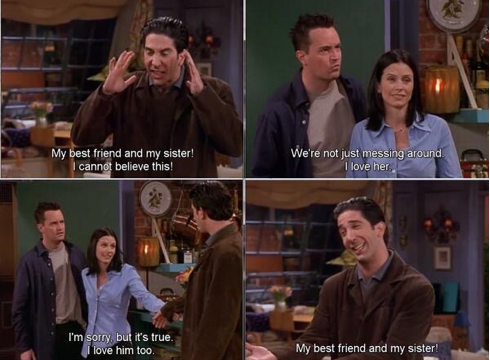
\includegraphics[width=0.9\textwidth]{figure/sisFri.png} 
  \caption{An example of communication with different expressions}
  \label{expression}
\end{figure}

% how to evaluate expression
Facial Action Coding System (FACS), developed by a Swedish anatomist named Carl-Herman Hjortsjö, is a system that classify the human facial movement by the appearance of the face ~\cite{facs70}. 


% The importance of privacy
\par
Door lock system through face recognition is a rapidly developed technology in security area. A potential vulnerable attacking method is reconstructing a 3D human face model through a video sequence which is definitely easy to get and then use the 3D printer to get a real face object which could be used to cheat the door lock system. 

Face recognition ATM



% pose
Pose estimation of faces are usually addressed assuming the face detection problem has been solved. 3D models and 2D view-based models are usually used. 


The essential of face de-identification problem is a face reconstruction process deleting the identity specific factors in the face.  
The key is how to build the database and train. 

The result of our project would be a synthetic face that would not be recognized by automatic face recognition algorithm but would be figured out by expression recognition algorithm. We are going to build a model with three kinds of parameters: identity, pose, expressions. 

A question: the appearance of a face. The result would be nobody, but it looks natural like the normal people. Why would it looks like a normal person?

Make it clear what data utility is. 

The problem is difficult as the appearance of a face could vary greatly due to the environmental factors like illumination and image noise or resolution. 

\section{Objectives}
We wish to create a new face model in which all identity factors are extracted independently and then reconstruct the face image with the de-identified identity facotrs. 

% Contribution
\section{Contributions}
\par


% Structure of the whole thesis
\section{Outline of this thesis}
\par 
The rest of this thesis is arranged as follows. 